\chapter{Lösungsansätze für Vier Gewinnt}

\section{Optimale Strategien}
Die Analyse von 4Gewinnt aus der Perspektive der Spieltheorie zeigt eine Reihe von strategischen Prinzipien und optimalen Spielweisen um gezielte Strategien zu entwickeln. Diese Erkenntnisse beruhen sowohl auf grundlegenden Prinzipien, welche in Kapitel 3 aufgearbeitet wurden, als auch auf fortgeschrittenen Taktiken, die im Verlauf des Spiels entscheidend sein können.

Ein wichtiges Grundprinzip ist die Bedeutung des ersten Zuges. Es wurde festgestellt, dass der erste Spieler, wenn er perfekt spielt, immer gewinnen kann – vorausgesetzt, er wählt den besten Eröffnungszug. Der optimale Zug ist dabei, den ersten Stein in die Mitte zu setzen. Diese Eröffnung ermöglicht die beste Kontrolle über das Spielbrett und eröffnet viele Möglichkeiten für offensive und defensive Züge. Zieht der erste Spieler jedoch in eine der angrenzenden Spalten, führen beide Spieler bei optimalem Spiel zu einem Unentschieden. Alle anderen Eröffnungszüge gelten als weniger effektiv und führen, wenn der Gegner ebenfalls perfekt spielt, unweigerlich zur Niederlage des ersten Spielers.

Ein weiteres zentrales Prinzip ist die Kontrolle des Zentrums, die eine entscheidende Rolle spielt. Die Kontrolle über die mittleren drei Spalten (insbesondere c, d und e) ist strategisch besonders wichtig, da sie die besten Chancen für horizontale, vertikale und diagonale Gewinnreihen bietet. Auch die Spalten b und f – die zweite und vorletzte Spalte – sind wichtig, denn ohne sie kann der Spieler keine vollständigen diagonalen oder horizontalen Viererreihen bilden. Diese Kontrolle hilft nicht nur beim eigenen Spielaufbau, sondern schränkt auch die Möglichkeiten des Gegners ein.

Im Laufe des Spiels kommen zudem fortgeschrittene taktische Elemente ins Spiel. Eine wichtige Taktik ist die Schaffung von Zugzwang-Situationen, in denen der Gegner gezwungen wird, einen Zug zu machen, der seine eigene Position schwächt. Diese Situationen sind besonders am Ende des Spiels von Bedeutung, wenn nur noch wenige Felder zur Verfügung stehen und der Druck auf beide Spieler steigt. Eine weitere wichtige Taktik sind Fallenkombinationen, bei denen der Gegner durch clevere Kombinationen von Bedrohungen in eine Falle gelockt wird. Besonders wirkungsvoll sind Doppelfallen, bei denen zwei gleichzeitige Drohungen entstehen, die der Gegner nicht gleichzeitig abwehren kann. Auch Auffüllfallen sind relevant: Hier zwingt ein Spieler den Gegner durch einen Mangel an freien Feldern dazu, einen entscheidenden Stein in eine vorbereitete Blockade zu setzen.

Die spieltheoretische Analyse von „Vier Gewinnt“ wurde durch mathematische und computerbasierte Methoden weiter vertieft. Unabhängig voneinander fanden zwei Forscher eine vollständige Lösung für das Spiel. Victor Allis entwickelte 1988 einen speziellen Regelsatz zur systematischen Analyse, während James D. Allen 1990 Computerprogramme einsetzte, um das Spiel vollständig zu berechnen. Beide kamen unabhängig zum gleichen Schluss: Der erste Spieler kann bei optimalem Spiel und einer Eröffnung in der Mitte immer gewinnen. Diese Erkenntnis hat nicht nur wissenschaftliche Bedeutung, sondern bildet auch die Basis für die Entwicklung von Algorithmen, die in Computerprogrammen oder Robotersystemen verwendet werden, um das Spiel optimal zu spielen. \autocites{wikipedia_vier_gewinnt}

	
	\subsection*{Mögliche Startpositionen und Spielausgänge}
	
	\textbf{1. Startposition 4 (mittlere Spalte)}
	Wenn der erste Spieler in die mittlere Spalte setzt, hat er einen nachgewiesenen Vorteil und kann bei perfektem Spiel gewinnen. Diese Eröffnung maximiert die Kontrolle über das Spielfeld.

\begin{figure}[H]
	\centering
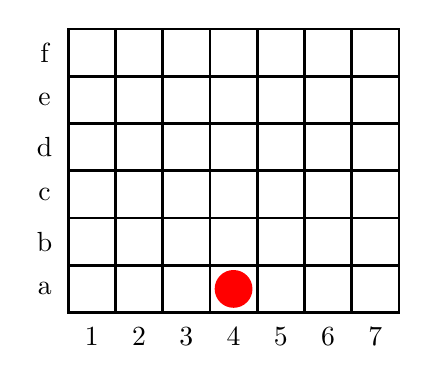
\begin{tikzpicture}[scale=0.6]
	% Zeichne das Gitter mit einheitlicher Linienstärke
	\foreach \x in {0,1,2,3,4,5,6} {
		\foreach \y in {0,1,2,3,4,5} {
			\draw[line width=1pt] (\x,\y) rectangle ++(1,1);
		}
	}
	
	% Beschriftung für Spalten (a-g)
	\foreach \x [count=\i from 1] in {1,2,3,4,5,6,7} {
		\node at (\i-0.5,-0.5) {\x};
	}
	
	% Beschriftung für Zeilen (1-6)
	\foreach \y [count=\j from 1] in {a,b,c,d,e,f} {
		\node at (-0.5,\j-0.5) {\y};
	}
	
	% Roter Stein in Feld d1 (Spalte d = 4, Zeile 1 = 0)
	\fill[red] (3.5,0.5) circle(0.4);
\end{tikzpicture}
  \caption{ROT gewinnt bei optimalen Spiel}
\label{fig:connect4_example}
\end{figure}

	
	
	\textbf{2. Startpositionen 3 oder 5 (benachbarte Spalten zur Mitte)}
	Ein Zug in die Spalte 3 oder 5 führt bei optimalem Spiel zu einem Remis, da der zweite Spieler durch eine Kombination aus Zentrums- und Blockstrategien den Sieg verhindern kann.
	
\begin{figure}[H]
	\centering
	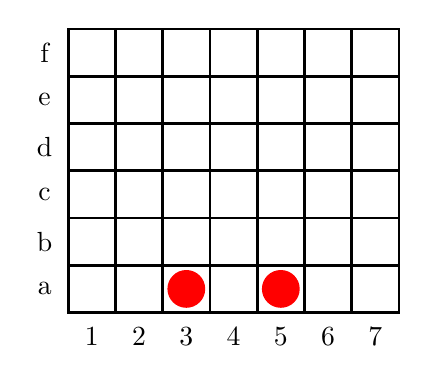
\begin{tikzpicture}[scale=0.6]
		% Zeichne das Gitter mit einheitlicher Linienstärke
		\foreach \x in {0,1,2,3,4,5,6} {
			\foreach \y in {0,1,2,3,4,5} {
				\draw[line width=1pt] (\x,\y) rectangle ++(1,1);
			}
		}
		
		% Beschriftung für Spalten (a-g)
		\foreach \x [count=\i from 1] in {1,2,3,4,5,6,7} {
			\node at (\i-0.5,-0.5) {\x};
		}
		
		% Beschriftung für Zeilen (1-6)
		\foreach \y [count=\j from 1] in {a,b,c,d,e,f} {
			\node at (-0.5,\j-0.5) {\y};
		}
		
		% Roter Stein in Feld d1 (Spalte d = 4, Zeile 1 = 0)
		\fill[red] (2.5,0.5) circle(0.4);
		\fill[red] (4.5,0.5) circle(0.4);
	\end{tikzpicture}
	\caption{Remis bei optimalen Spiel}
\end{figure}
	
	\textbf{3. Startpositionen 1, 2, 6 oder 7 (äußere Spalten)}
	Züge in die äußeren Spalten gelten als suboptimal. Der erste Spieler verliert bei perfektem Gegenspiel des zweiten Spielers, da diese Positionen weniger Kontrolle über das Zentrum und die Gewinnlinien bieten.
	
	\begin{figure}[H]
		\centering
		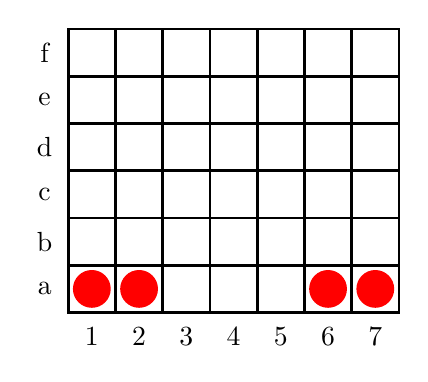
\begin{tikzpicture}[scale=0.6]
			% Zeichne das Gitter mit einheitlicher Linienstärke
			\foreach \x in {0,1,2,3,4,5,6} {
				\foreach \y in {0,1,2,3,4,5} {
					\draw[line width=1pt] (\x,\y) rectangle ++(1,1);
				}
			}
			
			% Beschriftung für Spalten (a-g)
			\foreach \x [count=\i from 1] in {1,2,3,4,5,6,7} {
				\node at (\i-0.5,-0.5) {\x};
			}
			
			% Beschriftung für Zeilen (1-6)
			\foreach \y [count=\j from 1] in {a,b,c,d,e,f} {
				\node at (-0.5,\j-0.5) {\y};
			}
			
			% Roter Stein in Feld d1 (Spalte d = 4, Zeile 1 = 0)
			\fill[red] (0.5,0.5) circle(0.4);
			\fill[red] (1.5,0.5) circle(0.4);
			\fill[red] (5.5,0.5) circle(0.4);
			\fill[red] (6.5,0.5) circle(0.4);
		\end{tikzpicture}
		\caption{ROT verliert bei optimalen Spiel}
	\end{figure}
	
	
	
	Diese Analyse zeigt, wie wichtig die Wahl der Startposition für den weiteren Spielverlauf ist. Der erste Zug in die Mitte eröffnet dem Spieler die besten Chancen, während Züge in die äußeren Spalten zu deutlichen Nachteilen führen können.

\section{Heuristische Ansätze}

Die Bewertung von Positionen auf dem Spielfeld ist ein zentraler heuristischer Ansatz bei der Strategieentwicklung für 4Gewinnt. Dieser Ansatz zielt darauf ab, den strategischen Wert jeder Position zu analysieren und darauf aufbauend optimale Züge zu planen.

Die dargestellte Tabelle veranschaulicht die strategische Bewertung jedes Spielfelds. Jedes Feld erhält einen numerischen Wert, der angibt, wie viele mögliche Viererreihen dieses Feld beeinflussen kann. Ein Zug auf ein Feld mit einem höheren Wert ist in der Regel strategisch besser, da er potenziell mehr Siegoptionen eröffnet. Solche Bewertungsansätze werden auch in computergesteuerten Spielen angewendet, um optimale Züge zu berechnen.

	
\begin{figure}[H]
	\centering
	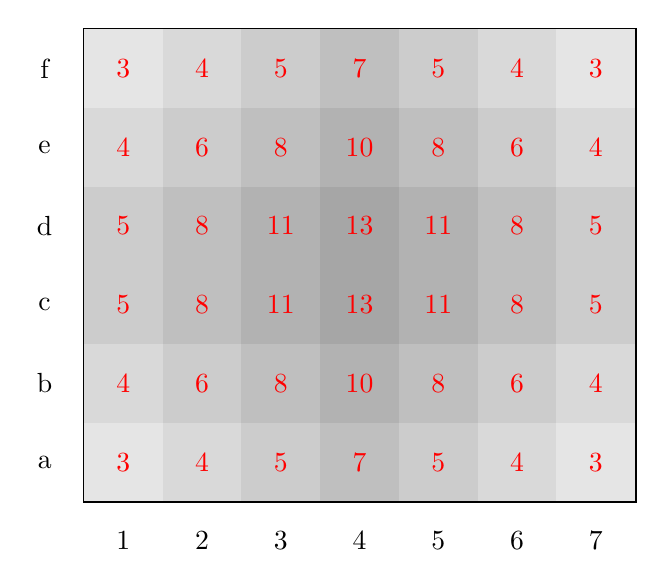
\begin{tikzpicture}[scale=1]
		% Zeichne das Gitter mit einheitlicher Linienstärke
		\foreach \x in {0,1,2,3,4,5,6} {
		\foreach \y in {0,1,2,3,4,5} {
			\draw[line width=1pt] (\x,\y) rectangle ++(1,1);
		}
	}
	
	% Beschriftung für Spalten (1-7)
	\foreach \x [count=\i from 1] in {1,2,3,4,5,6,7} {
		\node at (\i-0.5,-0.5) {\x};
	}
	
	% Beschriftung für Zeilen (a-f)
	\foreach \y [count=\j from 1] in {a,b,c,d,e,f} {
		\node at (-0.5,\j-0.5) {\y};
	}
		
		% Zahlen aus der Tabelle in die Felder einfügen und die Felder einfärben
		% Zeile 0
		\fill[gray!20] (0,5) rectangle ++(1,1); \node[red] at (0.5,5.5) {3};
		\fill[gray!30] (1,5) rectangle ++(1,1); \node[red] at (1.5,5.5) {4};
		\fill[gray!40] (2,5) rectangle ++(1,1); \node[red] at (2.5,5.5) {5};
		\fill[gray!50] (3,5) rectangle ++(1,1); \node[red] at (3.5,5.5) {7};
		\fill[gray!40] (4,5) rectangle ++(1,1); \node[red] at (4.5,5.5) {5};
		\fill[gray!30] (5,5) rectangle ++(1,1); \node[red] at (5.5,5.5) {4};
		\fill[gray!20] (6,5) rectangle ++(1,1); \node[red] at (6.5,5.5) {3};
		
		% Zeile 1
		\fill[gray!30] (0,4) rectangle ++(1,1); \node[red] at (0.5,4.5) {4};
		\fill[gray!40] (1,4) rectangle ++(1,1); \node[red] at (1.5,4.5) {6};
		\fill[gray!50] (2,4) rectangle ++(1,1); \node[red] at (2.5,4.5) {8};
		\fill[gray!60] (3,4) rectangle ++(1,1); \node[red] at (3.5,4.5) {10};
		\fill[gray!50] (4,4) rectangle ++(1,1); \node[red] at (4.5,4.5) {8};
		\fill[gray!40] (5,4) rectangle ++(1,1); \node[red] at (5.5,4.5) {6};
		\fill[gray!30] (6,4) rectangle ++(1,1); \node[red] at (6.5,4.5) {4};
		
		% Zeile 2
		\fill[gray!40] (0,3) rectangle ++(1,1); \node[red] at (0.5,3.5) {5};
		\fill[gray!50] (1,3) rectangle ++(1,1); \node[red] at (1.5,3.5) {8};
		\fill[gray!60] (2,3) rectangle ++(1,1); \node[red] at (2.5,3.5) {11};
		\fill[gray!70] (3,3) rectangle ++(1,1); \node[red] at (3.5,3.5) {13};
		\fill[gray!60] (4,3) rectangle ++(1,1); \node[red] at (4.5,3.5) {11};
		\fill[gray!50] (5,3) rectangle ++(1,1); \node[red] at (5.5,3.5) {8};
		\fill[gray!40] (6,3) rectangle ++(1,1); \node[red] at (6.5,3.5) {5};
		
		% Zeile 3
		\fill[gray!40] (0,2) rectangle ++(1,1); \node[red] at (0.5,2.5) {5};
		\fill[gray!50] (1,2) rectangle ++(1,1); \node[red] at (1.5,2.5) {8};
		\fill[gray!60] (2,2) rectangle ++(1,1); \node[red] at (2.5,2.5) {11};
		\fill[gray!70] (3,2) rectangle ++(1,1); \node[red] at (3.5,2.5) {13};
		\fill[gray!60] (4,2) rectangle ++(1,1); \node[red] at (4.5,2.5) {11};
		\fill[gray!50] (5,2) rectangle ++(1,1); \node[red] at (5.5,2.5) {8};
		\fill[gray!40] (6,2) rectangle ++(1,1); \node[red] at (6.5,2.5) {5};
		
		% Zeile 4
		\fill[gray!30] (0,1) rectangle ++(1,1); \node[red] at (0.5,1.5) {4};
		\fill[gray!40] (1,1) rectangle ++(1,1); \node[red] at (1.5,1.5) {6};
		\fill[gray!50] (2,1) rectangle ++(1,1); \node[red] at (2.5,1.5) {8};
		\fill[gray!60] (3,1) rectangle ++(1,1); \node[red] at (3.5,1.5) {10};
		\fill[gray!50] (4,1) rectangle ++(1,1); \node[red] at (4.5,1.5) {8};
		\fill[gray!40] (5,1) rectangle ++(1,1); \node[red] at (5.5,1.5) {6};
		\fill[gray!30] (6,1) rectangle ++(1,1); \node[red] at (6.5,1.5) {4};
		
		% Zeile 5
		\fill[gray!20] (0,0) rectangle ++(1,1); \node[red] at (0.5,0.5) {3};
		\fill[gray!30] (1,0) rectangle ++(1,1); \node[red] at (1.5,0.5) {4};
		\fill[gray!40] (2,0) rectangle ++(1,1); \node[red] at (2.5,0.5) {5};
		\fill[gray!50] (3,0) rectangle ++(1,1); \node[red] at (3.5,0.5) {7};
		\fill[gray!40] (4,0) rectangle ++(1,1); \node[red] at (4.5,0.5) {5};
		\fill[gray!30] (5,0) rectangle ++(1,1); \node[red] at (5.5,0.5) {4};
		\fill[gray!20] (6,0) rectangle ++(1,1); \node[red] at (6.5,0.5) {3};
		
	\end{tikzpicture}
	\caption{Bewertungstabelle: mögliche Anzahl an Vierer-Reihen}

\end{figure}
	
	\subsection*{Erklärung der Werte:}
	\textbf{Zentrum des Spielfelds:} Die Felder im Zentrum (insbesondere Spalte 4 und die Zeilen neben dran 3 und 5) haben die höchsten Werte, da sie Teil mehrerer potenzieller Viererreihen sein können – sowohl horizontal, vertikal als auch diagonal. Das erklärt, warum das Feld in Spalte 4, Zeilen c und d, den maximalen Wert von 13 besitzt.\\
	
	\textbf{Ränder des Spielfelds:} Die Felder am Rand (also die ersten und siebten Spalten sowie die Reihen a und f) zeigen deutlich niedrigere Werte. Das liegt daran, dass sie weniger Gewinnlinien bieten. Ein Randfeld kann höchstens Teil einer horizontalen und einer diagonalen Viererreihe sein, weshalb dort oft Werte von 3 oder 4 zu finden sind.
	
	\subsection*{Strategische Bedeutung:}
	Die zentralen Felder sind besonders wichtig, weil sie viele Optionen bieten, um eine Viererreihe zu vervollständigen. Deshalb ist es entscheidend, die mittleren Spalten – vor allem Spalte 4 sowie die angrenzenden Spalten 3 und 5 – im Auge zu behalten. Diese Kontrolle kann den Unterschied im Spiel ausmachen.
	Im Gegensatz dazu haben die Randfelder weniger Einfluss auf den Verlauf des Spiels. Sie werden oft hauptsächlich defensiv genutzt oder um den Gegner zu bestimmten Zügen zu zwingen.
	
	
\section{Entwicklung von Algorithmen}
In diesem Abschnitt werden verschiedene Algorithmen vorgestellt, die in unserem Projekt Anwendung finden können. Jeder Algorithmus wird zunächst in seinen Grundzügen erklärt, gefolgt von einer kritischen Bewertung zur Realisierung.
	
\subsection{MinMax-Algorithmus}

Die Minimax-Strategie ist ein grundlegender Algorithmus zur Entscheidungsfindung in Nullsummenspielen wie "Vier Gewinnt". Dieser Ansatz wird verwendet, um optimale Züge für einen Spieler zu finden, indem sowohl die eigenen Möglichkeiten als auch die möglichen Gegenreaktionen des Gegners analysiert werden. In diesem Kapitel betrachten wir die Funktionsweise der Minimax-Strategie im Kontext von "Vier Gewinnt" und zeigen, wie sie das Spielverhalten verbessern kann.

Grundprinzip der Minimax-Strategie

Der Minimax-Algorithmus funktioniert nach dem Prinzip der Maximierung des eigenen Nutzens und der Minimierung des Nutzens des Gegners. In einem Spielbaum, der alle möglichen Züge und Gegenreaktionen darstellt, sucht der Algorithmus nach dem optimalen Zug, indem er die Ergebnisse aller möglichen Züge bis zu einer bestimmten Tiefe bewertet.

In der Spieltheorie bezeichnet ein Spielbaum einen azyklischen, gerichteten Graphen, in dem die Knoten die verschiedenen Stellungen eines Spiels repräsentieren. Dabei kann dieselbe Stellung an mehreren Knoten des Spielbaums auftreten. Jeder Knoten kennzeichnet zudem, welcher Spieler in dieser Position am Zug ist. Der Spieler hat die Möglichkeit, eine der verfügbaren Aktionen auszuwählen, die durch die Kanten des Graphen dargestellt werden.

Jede Spielstellung im Baum ist entweder eine Endstellung oder besitzt eine Menge von Nachfolgestellungen, die durch die möglichen Züge im nächsten Halbzug des Spiels erreicht werden können.

Die Bewertung erfolgt durch eine sogenannte Heuristik, die den Wert eines Spielzustands quantifiziert. In "Vier Gewinnt" könnte eine einfache Heuristik beispielsweise folgende Aspekte bewerten:

\begin{itemize}
	\item Gewonnene Spiele: Ein Zustand, in dem ein Spieler vier Steine in einer Reihe hat, hat den höchsten Wert.
	\item Blockierte Gewinnchancen: Züge, die verhindern, dass der Gegner vier in einer Reihe erreicht, sind besonders wertvoll.
	\item Teilweise vervollständigte Reihen: Zustände, in denen drei oder zwei verbundene Steine existieren, sind wertvoller als isolierte Steine.
\end{itemize}

Der Algorithmus berechnet mögliche Züge und bewertet sie rückwärts ausgehend von den möglichen Endzuständen.

Maximierer und Minimierer

In "Vier Gewinnt" gibt es zwei Spieler:

\begin{itemize}
	\item Der Maximierer versucht, den eigenen Nutzen zu maximieren (z. B. Spieler 1).
	\item Der Minimierer versucht, den Nutzen des Gegners zu minimieren (z. B. Spieler 2).
\end{itemize}

Bei jedem Zug wechselt die Rolle zwischen Maximierer und Minimierer. Der Algorithmus wechselt daher bei jedem Ebenenwechsel zwischen der Maximierung und Minimierung der Heuristikwerte.

\section*{Beispiel: Minimax-Suchbaum}

Im Folgenden wird ein einfacher Suchbaum dargestellt, der die Funktionsweise des Minimax-Algorithmus illustriert. Der Baum hat eine Tiefe von 2 (eine Max-Ebene und eine Min-Ebene).

\subsection*{Suchbaum}

\begin{figure}[h!]
	\centering
	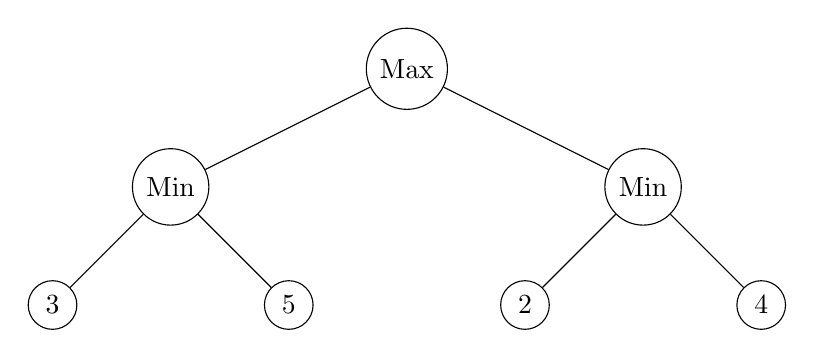
\begin{tikzpicture}[
		level distance=1.5cm,
		level 1/.style={sibling distance=6cm},
		level 2/.style={sibling distance=3cm},
		every node/.style={circle, draw, align=center}
		]
		\node {Max}
		child {node {Min}
			child {node {3}}
			child {node {5}}
		}
		child {node {Min}
			child {node {2}}
			child {node {4}}
		};
	\end{tikzpicture}
	\caption{Ein einfacher Minimax-Suchbaum mit einer Tiefe von 2.}
	\label{fig:minimax-example}
\end{figure}

\subsection*{Erklärung des Suchbaums}

Der Suchbaum in Abbildung \ref{fig:minimax-example} zeigt die Schritte des Minimax-Algorithmus:

\begin{enumerate}
	\item \textbf{Blattebene:} Die unterste Ebene enthält die Bewertungen der möglichen Endzustände aus Sicht des Max-Spielers. Diese Werte könnten durch eine Bewertungsfunktion ermittelt worden sein.
	\begin{itemize}
		\item Die Knoten haben die Werte 3, 5, 2 und 4.
	\end{itemize}
	
	\item \textbf{Min-Ebene:} Der Min-Spieler versucht, die Bewertung zu minimieren. Für jeden Min-Knoten wird der niedrigste Wert seiner Kindknoten ausgewählt:
	\begin{itemize}
		\item Der linke Min-Knoten wählt $\min(3, 5) = 3$.
		\item Der rechte Min-Knoten wählt $\min(2, 4) = 2$.
	\end{itemize}
	
	\item \textbf{Max-Ebene:} Der Max-Spieler versucht, die Bewertung zu maximieren. Der Max-Knoten wählt den höchsten Wert aus den zurückgegebenen Bewertungen der Min-Knoten:
	\begin{itemize}
		\item Der Max-Knoten wählt $\max(3, 2) = 3$.
	\end{itemize}
\end{enumerate}

\subsection*{Optimale Entscheidung}

Der optimale Zug für den Max-Spieler ist derjenige, der zu einer Bewertung von \textbf{3} führt.

\subsection*{Zusammenfassung}

Der Minimax-Algorithmus analysiert den Baum von unten nach oben:
\begin{itemize}
	\item Min-Knoten repräsentieren die Entscheidungen des Gegners (Minimierer).
	\item Max-Knoten repräsentieren die Entscheidungen des Spielers (Maximierer).
\end{itemize}

Durch diese systematische Analyse findet der Algorithmus den besten Zug für den Maximierer unter der Annahme, dass der Minimierer optimal spielt.



\subsection{AlphaBeta-Algorithmus}

Der Alpha-Beta-Algorithmus ist eine Optimierung des Minimax-Algorithmus, die dessen Effizienz erheblich steigert. Durch das gezielte Verwerfen von Spielzügen, die für die Entscheidung irrelevant sind, reduziert der Alpha-Beta-Algorithmus die Anzahl der bewerteten Knoten im Spielbaum. Diese Technik ist besonders wertvoll bei ressourcenbeschränkten Systemen wie einem LEGO Spike Roboter, der begrenzte Rechenleistung zur Verfügung hat.

Der Alpha-Beta-Algorithmus führt die gleichen Berechnungen wie der Minimax-Algorithmus durch, ergänzt jedoch zwei zusätzliche Parameter, Alpha und Beta, um unnötige Berechnungen zu vermeiden:

\begin{itemize}
	\item \textbf{Alpha}: Der aktuelle maximale Wert, den der Maximierer sicher erreichen kann.
	\item \textbf{Beta}: Der aktuelle minimale Wert, den der Minimierer sicher erreichen kann.
\end{itemize}

Während der Traversierung des Spielbaums werden Äste abgeschnitten, die keine Auswirkungen auf die endgültige Entscheidung haben (\textit{Pruning}). Dies geschieht, wenn:
\begin{itemize}
	\item Ein Knoten einen Wert liefert, der schlechter ist als der bisher bekannte Alpha-Wert für den Maximierer.
	\item Ein Knoten einen Wert liefert, der schlechter ist als der bisher bekannte Beta-Wert für den Minimierer.
\end{itemize}

Die Anwendung des Alpha-Beta-Algorithmus auf "Vier Gewinnt" bietet mehrere Vorteile:
\begin{itemize}
	\item \textbf{Effizienz}: Der Algorithmus reduziert die Anzahl der Knoten, die bewertet werden müssen, erheblich. Dies ermöglicht die Analyse tieferer Spielbäume mit derselben Rechenleistung.
	\item \textbf{Flexibilität}: Der Algorithmus kann leicht an die spezifische Bewertungsfunktion von "Vier Gewinnt" angepasst werden, z. B. zur Bewertung von Reihen, Spalten und Diagonalen.
	\item \textbf{Optimierung für begrenzte Ressourcen}: Ein LEGO Spike Roboter hat begrenzte Rechen- und Speicherkapazitäten. Der Alpha-Beta-Algorithmus ermöglicht es, in Echtzeit Züge zu berechnen, ohne den Roboter zu überlasten.
\end{itemize}

\section*{Beispiel: Alpha-Beta-Suchbaum}

Im Folgenden wird ein einfacher Suchbaum dargestellt, der die Funktionsweise des Alpha-Beta-Algorithmus illustriert. Der Baum zeigt, wie bestimmte Zweige (\textit{Pruning}) abgeschnitten werden, um die Effizienz zu erhöhen.

\subsection*{Suchbaum mit Alpha-Beta-Pruning}

\begin{figure}[h!]
	\centering
	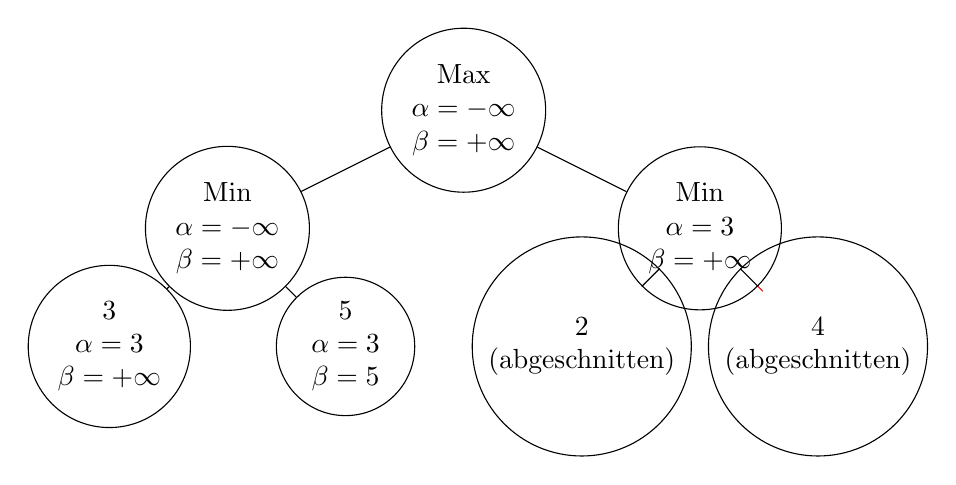
\begin{tikzpicture}[
		level distance=1.5cm,
		level 1/.style={sibling distance=6cm},
		level 2/.style={sibling distance=3cm},
		every node/.style={circle, draw, align=center}
		]
		% Root level (Max)
		\node (A) {Max\\$\alpha = -\infty$\\$\beta = +\infty$}
		% Left subtree (Min)
		child {node (B) {Min\\$\alpha = -\infty$\\$\beta = +\infty$}
			child {node {3\\$\alpha = 3$\\$\beta = +\infty$}}
			child {node {5\\$\alpha = 3$\\$\beta = 5$}}
		}
		% Right subtree (Min)
		child {node (C) {Min\\$\alpha = 3$\\$\beta = +\infty$}
			child {node {2\\(abgeschnitten)}}
			child {node {4\\(abgeschnitten)}}
		};
		% Pruning lines
		\draw[dashed, red] (C) -- +(0.8,-0.8);
	\end{tikzpicture}
	\caption{Ein Alpha-Beta-Suchbaum mit Pruning. Zweige werden abgeschnitten, wenn sie die Grenzen von Alpha und Beta verletzen.}
	\label{fig:alphabeta-example}
\end{figure}

\subsection*{Erklärung des Suchbaums}

Der Suchbaum in Abbildung \ref{fig:alphabeta-example} zeigt die Schritte des Alpha-Beta-Algorithmus:

\begin{enumerate}
	\item \textbf{Initialisierung:} Die Alpha- und Beta-Werte werden am Wurzelknoten initialisiert:
	\begin{itemize}
		\item $\alpha = -\infty$: Das beste Ergebnis, das der Maximierer bisher erreicht hat.
		\item $\beta = +\infty$: Das schlechteste Ergebnis, das der Minimierer dem Maximierer erlauben würde.
	\end{itemize}
	
	\item \textbf{Linker Teilbaum:} 
	\begin{itemize}
		\item Der Maximierer überprüft den linken Teilbaum, in dem der Minimierer aktiv ist.
		\item Der Min-Knoten prüft seine Kindknoten:
		\begin{itemize}
			\item Der erste Kindknoten liefert den Wert 3. Der Alpha-Wert wird aktualisiert: $\alpha = 3$.
			\item Der zweite Kindknoten liefert den Wert 5. Da 5 größer ist, bleibt $\alpha = 3$ bestehen.
		\end{itemize}
	\end{itemize}
	
	\item \textbf{Rechter Teilbaum (Pruning):}
	\begin{itemize}
		\item Der Maximierer prüft den rechten Teilbaum. Der Min-Knoten beginnt mit der Analyse.
		\item Bereits beim ersten Kindknoten erkennt der Algorithmus, dass dessen Wert (2) kleiner ist als $\alpha = 3$.
		\item Alle verbleibenden Kindknoten des rechten Teilbaums werden abgeschnitten (\textit{Pruning}), da sie keinen besseren Wert liefern können.
	\end{itemize}
\end{enumerate}

\subsection*{Vorteile des Alpha-Beta-Algorithmus}

Durch das Alpha-Beta-Pruning werden unnötige Berechnungen vermieden:
\begin{itemize}
	\item Der Algorithmus durchsucht nur jene Zweige, die potenziell zu besseren Ergebnissen führen.
	\item In diesem Beispiel werden zwei Knoten (Wert 2 und 4 im rechten Teilbaum) nicht berechnet.
	\item Dies erhöht die Effizienz und ermöglicht es, tiefere Suchbäume mit derselben Rechenleistung zu analysieren.
\end{itemize}